\documentclass[t]{beamer}

%\documentclass[handout, t]{beamer}
\setbeamertemplate{navigation symbols}{}
\usepackage{pstricks}
\usepackage{mathtools}
\usepackage{amsfonts}
\usepackage{mathrsfs}
\usepackage{amsmath}
\setbeamertemplate{navigation symbols}{}
\usepackage{bm}
\usepackage[UTF8]{ctex}
\usetheme{AnnArbor}
\usefonttheme{serif}
\useinnertheme{rounded}
%\usecolortheme{crane}
\setbeamertemplate{blocks}[rounded][shadow=true]

\newcommand{\dif}{{\;\rm d}}
\usepackage{graphicx}
\usepackage{pgf}
\usepackage{tikz}
\usetikzlibrary{arrows, decorations.pathmorphing, backgrounds, positioning, fit, petri, automata}
\tikzset{>=stealth}

\usepackage{setspace}
\setmainfont{Times New Roman}
\setCJKmainfont{Microsoft YaHei}


\hypersetup{pdfpagemode=FullScreen}
\renewcommand{\Pr}{\mathbb{P}}
\usepackage{blkarray}


\setbeamercolor{block title}{bg=red!10!white}
\setbeamercolor{block body}{bg=gray!10!white}

\usepackage{multicol}
\newcommand{\E}{\mathbb{E}}
\newcommand{\EP}{\mathbb{E}^{\mathbb{P}}}
\newcommand{\EQ}{\mathbb{E}^{\mathbb{Q}}}
\newcommand{\Var}{{\rm Var}}
\newcommand{\Cov}{{\rm Cov}}


\begin{document}
\fontsize{11}{18}\selectfont


\CTEXindent



  \title{第三章~~可数状态马氏链}
\author{应用随机过程}
\date{中国人民大学出版社}
  \begin{frame}
    \maketitle
  \end{frame}

  \begin{frame}{离散时间马氏链与可数状态马氏链}
    离散时间马氏链的时间和状态均离散,并且状态是有限的。
    
    本章将在其基础上,将状态空间拓展为可数(countable)状态。所谓的可数状态是指状态的取值是在整数域$\mathbb{Z}$上,且状态的数量无穷大,因此可数状态马氏链所包含的状态为:$S=\mathbb{Z}$。正因为可数状态马氏链的状态数是无穷多个,其与离散时间马氏链在性质上存在一定的区别。
  \end{frame}

\begin{frame}{本章内容}
    \tableofcontents
\end{frame}

\section{状态的分类}
\begin{frame}{状态的分类}
    可数状态马氏链遇到的新问题是常返并不能保证平稳分布的存在。与离散时间马氏链不同,可数状态马氏链中的状态分为三大类:正常返、零常返和非常返。
\end{frame}



\begin{frame}{举例1:带反射壁的随机游动}
    质点在$\{0,1,2,\ldots\}$上游动,它以概率$p$向右移动一步,以概率$(1-p)$向左移动一步,但是如果处于0点,并试图向左移动一步时,它将停留在0点。
    \begin{center}
    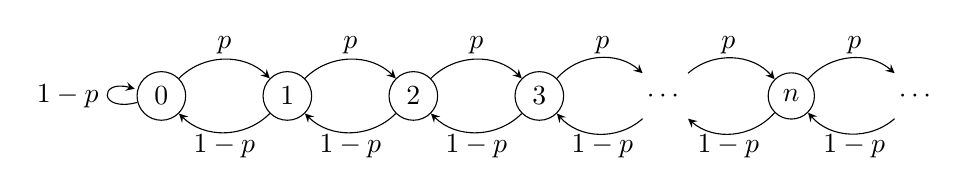
\begin{tikzpicture}[>=stealth, scale=.8]
    \node (A) [draw, circle] at (0,0) {0};
    \node (B) [draw, circle] at (2,0) {1};
    \node (C) [draw, circle] at (4,0) {2};
    \node (D) [draw, circle] at (6,0) {3};
    \node (E) [circle] at (8,0) {$\cdots$};
    \node (F) [draw, circle] at (10,0) {$n$};
    \node (G) [circle] at (12,0) {$\cdots$};
    
    \draw [->](A)  [bend left =45] to (B);
    \draw [->](B)  [bend left =45] to (A);
    \draw [->](B)  [bend left =45] to (C);
    \draw [->](C)  [bend left =45] to (B);
    \draw [->](C)  [bend left =45] to (D);
    \draw [->](D)  [bend left =45] to (C);
    \draw [->](D)  [bend left =45] to (E);
    \draw [->](E)  [bend left =45] to (D);
    \draw [->](E)  [bend left =45] to (F);
    \draw [->](F)  [bend left =45] to (E);
    \draw [->](F)  [bend left =45] to (G);
    \draw [->](G)  [bend left =45] to (F);
    
    \node at (1,.8){$p$};
    \node at (1,-.8){$1-p$};
    \node at (3,.8){$p$};
    \node at (3,-.8){$1-p$};
    \node at (5,.8){$p$};
    \node at (5,-.8){$1-p$};
    \node at (7,.8){$p$};
    \node at (7,-.8){$1-p$};
    \node at (9,.8){$p$};
    \node at (9,-.8){$1-p$};
    \node at (11,.8){$p$};
    \node at (11,-.8){$1-p$};
    \path (A) edge [loop left] node[left] {$1-p$} (A);
    \end{tikzpicture}    
\end{center}

\end{frame}


\begin{frame}{带反射壁的随机游动(cont.)}
    相应的转移概率如下:
    \[p(0,0)=1-p,\qquad \begin{cases}
    p(i,i+1)=p,&i\ge 0\\
    p(i,i-1)=1-p,&i\ge 1\\
    \end{cases}
     \]
    
    该模型属于生灭链的特殊形式,可以根据细致平衡方程来求其平稳分布
    \[\begin{split}
    p(i,j)\pi(i)&=p(j,i)\pi(j)\\
    p(i,i+1)\pi(i)&=p(i+1,i)\pi(i+1),\qquad i\ge 0\\
    p\cdot \pi(i)&=(1-p)\cdot \pi(i+1)
    \end{split} \]
    因此:\[\pi(i+1)=\frac{p}{1-p}\pi(i) \]
\end{frame}


\begin{frame}{带反射壁的随机游动(cont.)}
    令$\pi(0)=c$,则:
    \[\pi(i)=\pi(0)\left(\frac{p}{1-p}\right)^i =c\left(\frac{p}{1-p}\right)^i \]
    注意到,当$p/(1-p)<1$时,$p<1/2$,此时:
    \[\sum_{i=0}^{\infty}\pi(i)=c\sum_{i=0}^{\infty}\left(\frac{p}{1-p}\right)^i=\frac{c}{1-\dfrac{p}{1-p}}=\frac{1-p}{1-2p}c<\infty \]
    对于平稳分布而言,必须满足$\displaystyle\sum_{i=0}^{\infty}\pi(i)=1$,因此:
    \[c=\frac{1-2p}{1-p} \]
\end{frame}


\begin{frame}{带反射壁的随机游动(cont.)}
    从而:\[\pi(i)=\frac{1-2p}{1-p}\cdot \left(\frac{p}{1-p}\right)^i \]
    因此:$$\E_0(\tau_0)=\frac{1}{\pi(0)}=\frac{1-p}{1-2p}<\infty $$
    称状态0是{正常返}(positive recurrent)的。因此$p<1/2$时,该马氏链是正常返的,且存在一个平稳分布$\pi(i)$。

    \begin{block}{注意:}
       对正常返的马氏链,一定可以找到其对应的平稳分布;若马氏链不存在平稳分布,则其可能是零常返(null recurrent)或非常返的。
    \end{block}
\end{frame}


\begin{frame}{带反射壁的随机游动(cont.)}
\[\pi(i)=c\left(\frac{p}{1-p}\right)^i,\qquad c=\frac{1-2p}{1-p} \]

\begin{itemize}
    \item 当$p>1/2$时,$p/(1-p)>1, c<0$,此时$\{\pi(i)\}$序列是发散的(即 $|\pi(i+1)|>|\pi(i)|$),因而不存在平稳分布,此时马氏链是{非常返}的。
    \item 当$p=1/2$时,$p/(1-p)=1,\; c=0$,此时$\pi(i)=0,\; \forall i$,相应地:
        $$\E_x(\tau_x)=\frac{1}{\pi(x)}=\infty$$
    而$\displaystyle\sum_{i=0}^{\infty}\pi(i)=1$, 
        因而不存在平稳分布,此时马氏链的各状态均是{零常返}态。
\end{itemize}
\end{frame}


\begin{frame}{状态的判定}
    零常返态代表了常返态和非常返态的边界情况。
    三者的联系和区别具体体现在:
    \begin{enumerate}
        \item 正常返态:$\Pr_x(\tau_x<\infty)=1, \; \E_x(\tau_x)<\infty$;
    \item	零常返态:$\Pr_x(\tau_x<\infty)=1, \;\E_x(\tau_x)=\infty$;
    \item 非常返态:$\Pr_x(\tau_x<\infty)<1, \;\E_x(\tau_x)=\infty$。
    \end{enumerate}
\end{frame}

\section{分支过程}

\begin{frame}{分支过程}
    在可数状态马氏链的相关研究中,有一类非常重要的随机过程常常应用于生物学领域,这就是分支过程(branching process)。分支过程最早由弗朗西斯·高尔顿(Francis  Galton)和沃森(Watson)提出,用于对姓氏消失现象的定量解释。后来该过程被用于生物种群消亡等问题的研究。
\end{frame}


\begin{frame}{分支过程举例}
    考虑一个家族的第$n$代每一个个体产生后代的个数$Y_1,Y_2,\ldots$都相互独立同分布,并且每个个体产生$k$个后代的概率均是$p_k=p(1,k)$。第$n$代的个体数$X_n$是一个马氏链,其状态空间为$\{0,1,2,\ldots\}$,其转移概率如下:
    \[p(i,j)=\Pr(Y_1+Y_2+\cdots+Y_i=j),\qquad i>0,\; j\ge 0 \]
    问:该家族避免消亡的概率是多少?

    \begin{block}{思路:}
        此处的“消亡”是指马氏链吸收于状态0。
    \end{block}
\end{frame}




\begin{frame}{分支过程举例(cont.)}
    该家族的消亡发生与否,可通过一个个体的平均后代数量$\mu$来确定:
    \[\mu=\sum_{k=0}^{\infty}k\cdot p(1,k)=\sum_{k=0}^{\infty}k\cdot p_k \]
    由于$X_n$表示第$n$代的个体数,因此:
    \[\E(X_n|X_{n-1})=\mu X_{n-1} \quad \Rightarrow\quad \E(X_n)=\mu\E(X_{n-1}) \]
    通过迭代可得:\[\E(X_n)=\mu^{n}\E(X_0) \]
    显然,{$\mu<1$时,$\lim\limits_{n\to\infty}\E(X_n)=0$,该家族以概率1消亡。}
\end{frame}


\begin{frame}{$\mu\ge1$的情形}
    引入消亡概率(extinction probability),记作$\alpha$,表示当前时刻的某个个体在未来的消亡概率。\footnote{这里的消亡概率,可以理解为个体因疾病、衰老等原因死亡的概率。}
    即:$$\alpha=\Pr(\tau_0<\infty|X_0=1)$$
    其中$\tau_0$表示个体全部消亡的时刻。如果当前时刻有$k$个个体,则他们全部消亡的概率是$\alpha^k$,因此:
    \[\alpha=\Pr(\tau_0<\infty|X_0=1)=\sum^{\infty}_{k=0}p(1,k)\cdot {\Pr(\tau_0<\infty|X_1=k)}
    \]

    最终可得:
\begin{equation*}
\alpha=\sum^{\infty}_{k=0}p_k\cdot {\alpha^k} 
\end{equation*}
\end{frame}


\begin{frame}{$\mu\ge1$的情形(cont.)}
\[\alpha=\sum^{\infty}_{k=0}p_k\cdot {\alpha^k} 
\]
记$G(\alpha)=\displaystyle\sum^{\infty}_{k=0}p_k\alpha^k$,则上式可表示为:$G(\alpha)=\alpha$

当$\alpha=0$和$\alpha=1$时,等式左侧分别为:
\[G(0)=p_0=p(1,0), \qquad 
G(1)=\sum^{\infty}_{k=0}p_k=1
\]
\begin{block}{注意:}
    $\alpha=1$是$G(\alpha)=\alpha$的平凡解(trivial solution)。要求的消亡概率$\alpha$应当是$G(\alpha)=\alpha$所有根当中的最小正根。
\end{block}
\end{frame}


\begin{frame}{$\mu\ge1$的情形(cont.)}
    对$G(\alpha)=\displaystyle\sum^{\infty}_{k=0}p_k\alpha^k$关于$\alpha$求一阶和二阶导,可得:
    \begin{equation*}
        G'(\alpha)=\sum^{\infty}_{k=0}k\cdot  p_k \alpha^{k-1}\ge 0,\qquad 
        G''(\alpha)=\sum^{\infty}_{k=1}k(k-1)\cdot  p_k \alpha^{k-2}\ge 0
        \end{equation*}
        由此可见,函数$G(\alpha)$是凸向原点的单调递增曲线。
        
        当$\alpha=1$时:
$$G'(1)=\sum^{\infty}_{k=0}k\cdot  p_k =\mu>0$$        
\end{frame}


\begin{frame}{两种可能性}
    \begin{tikzpicture}[>=stealth,scale=.8]
        \draw [->](0,0)--(5,0);
        \draw [->](0,0)--(0,5);
        \draw [dashed] (4,0)--(4,4)--(0,4);
        \draw [very thick](0,0)--(4,4);
        \node at (0,4)[left]{1};
        \node at (4,0)[below]{1};
        \node at (0,0)[below]{0};
        \node at (0,4.75)[right]{$G(\alpha)$};
        \node at (5,0)[above]{$\alpha$};
        \draw  [very thick] (0,1.5) to [bend right=10] (4,4);
        \node at (0,1.5)[left]{$p_0$};
        
        \node at (2,-.5){(a)};
        \end{tikzpicture}\quad 
        \begin{tikzpicture}[>=stealth,scale=.8]
        \draw [->](0,0)--(5,0);
        \draw [->](0,0)--(0,5);
        \draw [dashed] (4,0)--(4,4)--(0,4);
        \draw [very thick](0,0)--(4,4);
        \node at (0,4)[left]{1};
        \node at (4,0)[below]{1};
        \node at (0,0)[below]{0};
        \node at (0,4.75)[right]{$G(\alpha)$};
        \node at (5,0)[above]{$\alpha$};
        \draw  [very thick] (0,1) to [bend right] (4,4);
        \node at (0,1)[left]{$p_0$};
        \node at (1.3,0)[below]{$\alpha^*$};
        \draw [dashed] (1.3,0)--(1.3,1.3)--(0,1.3);
        \fill  (1.3,1.3) circle (2pt);
        \node at (2,-.5){(b)};
        \end{tikzpicture}

        \begin{enumerate}
            \item $G'(1)<1$时,$\alpha=1$;
            \item $G'(1)>1$时,$\alpha<1$。
            \end{enumerate}
\end{frame}


\begin{frame}{分支过程的结论}
由于$G'(1)=\mu$,因此进一步可以得到如下结论:

若$\mu$表示一个个体的平均后代数量,则:
\begin{enumerate}
	\item 当$\mu\le 1$时,消亡以概率1发生;
	\item 当$\mu>1$时,存在一个正的概率避免消亡。
\end{enumerate}
\end{frame}


\begin{frame}{分支过程举例1}
    当$p_0=1/4$,$p_1=1/4$,$p_2=1/2$时,
\[\mu=\frac{1}{4}\times 1+\frac{1}{2}\times 2=1.25>1\]
因此:消亡概率不为1。
    根据$G(\alpha)=\alpha$,可得:
	\[
G(\alpha)=p_0\alpha^0+p_1\alpha^1+p_2\alpha^2=\alpha \quad \Rightarrow\quad\frac{1}{2}\alpha^2+\left(\frac{1}{4}-1\right)\alpha+\frac{1}{4}=0
 \]
	$\alpha_1=1$或$\alpha_2=1/2$,最小正根是1/2。因此,$\alpha=0.5$,即消亡概率是0.5。
\end{frame}



\begin{frame}{分支过程举例2:二分支过程}
    当$p_0=1-a$,$p_2=a$,$p_k=0,\;k\ne 0,2$时,
    \[\mu=0(1-a)+2a=2a \]
因此,当$a\le \dfrac{1}{2}$时,消亡以概率1发生;
当$a> \dfrac{1}{2}$时,
    根据$G(\alpha)=\alpha$,可得:
    \[
    G(\alpha)=p_0\alpha^0+p_2\alpha^2=\alpha\quad \Rightarrow\quad 
        a\alpha^2-\alpha+(1-a)=0\]
    解得:$$\alpha_1=1\qquad \text{或}\qquad \alpha_2=\frac{1-a}{a}<1$$
此时消亡概率$\alpha=\dfrac{1-a}{a}$。

\end{frame}

\begin{frame}{二分支过程(cont.)}
最终结论:
    \begin{enumerate}
        \item 当$a>\dfrac{1}{2}$时,消亡以概率1发生;
        \item 当$a\le \dfrac{1}{2}$时,消亡概率$\alpha=\dfrac{1-a}{a}$。
    \end{enumerate}
\end{frame}




\begin{frame}{分支过程举例3:姓氏的消亡}
    高尔顿和沃森最初考虑的问题是人群中姓氏消亡的概率,而姓氏是由后代中的男性所继承,因此他们所研究的问题便转化为后代中男性消亡的概率。

    假设每个家庭都恰好有3个孩子,并且每个母亲平均有1.5个女儿,计算一个妇女
    的后代当中,男性消亡的概率。
\end{frame}


\begin{frame}{姓氏的消亡(cont.)}
    男女的概率均为1/2;假设后代中有$k$个男性,则相应的概率分布如下:
    \[\begin{split}
    \Pr(k=0)&={3\choose 0}\left(\frac{1}{2}\right)^0\left(\frac{1}{2}\right)^3=\frac{1}{8},\quad
    \Pr(k=1)={3\choose 1}\left(\frac{1}{2}\right)^1\left(\frac{1}{2}\right)^2=\frac{3}{8}\\
    \Pr(k=2)&={3\choose 2}\left(\frac{1}{2}\right)^2\left(\frac{1}{2}\right)^1=\frac{3}{8},\quad
    \Pr(k=3)={3\choose 3}\left(\frac{1}{2}\right)^3\left(\frac{1}{2}\right)^0=\frac{1}{8}\\
    \end{split} \]
    由于平均男性后代数量为$\mu=1.5>1$,因此需要计算消亡概率。
\end{frame}


\begin{frame}{姓氏的消亡(cont.)}
    根据 $G(\alpha)=\displaystyle\sum_k \alpha^kp_k=\alpha$,可得:
    \[\begin{split}
    \alpha&= \alpha^0\cdot  \Pr(k=0)+\alpha^1\cdot  \Pr(k=1)+\alpha^2 \cdot \Pr(k=2)+\alpha^3\cdot \Pr(k=3) \\
    &=\frac{1}{8}+\frac{3}{8}\alpha+\frac{3}{8}\alpha^2+\frac{1}{8}\alpha^3
    \end{split}\]
    因此,$\alpha^3+3\alpha^2-5\alpha+1=0$。由于已知$\alpha=1$是一个平凡解,对刚才的多项式关于$(\alpha-1)$进行分解,可得:
    \[\alpha^3+3\alpha^2-5\alpha+1=(\alpha-1)(\alpha^2+4\alpha-1)=0 \]
    从而:\[\alpha_{1,2}=\frac{-4\pm\sqrt{16+4}}{2}=-2\pm\sqrt{5} \]
    其中小于1的正解为$\alpha=\sqrt{5}-2$,因此男性消亡的概率为$\sqrt{5}-2$。
\end{frame}




\end{document}